%%%%%%%%%%%%%%%%%%%%%%%%%%%%%%%%%%%%%%%%%%%%%%%%%%%%%%%%%%%%%%%%%%%%%%%%
% AAMAS 2027 main-track submission, GAAI area.
% Anonymous working draft derived from the evidence-frozen USENIX manuscript.
%%%%%%%%%%%%%%%%%%%%%%%%%%%%%%%%%%%%%%%%%%%%%%%%%%%%%%%%%%%%%%%%%%%%%%%%

% TeX Live 2017 does not preload the LaTeX3 command layer used by the 2027
% class. Loading it explicitly is a local toolchain compatibility measure; the
% official class and all layout parameters remain unchanged.
\RequirePackage{expl3}
\documentclass[sigconf,anonymous]{aamas}

\usepackage{balance}
\usepackage{amsmath}
% The class loads newtxmath, which already defines \Bbbk; without this guard
% current TeX Live stops with "Command \Bbbk already defined".
\let\Bbbk\relax
\usepackage{amssymb}
\usepackage{amsthm}
\usepackage{bm}
\usepackage{booktabs}
\usepackage{graphicx}
\usepackage{tikz}
\usetikzlibrary{arrows.meta,positioning,fit,calc}
\usepackage{pgfplots}
\pgfplotsset{compat=1.14}

\makeatletter
\gdef\@copyrightpermission{
  \begin{minipage}{0.2\columnwidth}
   \href{https://creativecommons.org/licenses/by/4.0/}{
\includegraphics[width=0.90\textwidth]{by}}
  \end{minipage}\hfill
  \begin{minipage}{0.8\columnwidth}
   \href{https://creativecommons.org/licenses/by/4.0/}{This work is licensed under a Creative Commons Attribution International 4.0 License.}
  \end{minipage}
  \vspace{5pt}
}
\makeatother

\setcopyright{ifaamas}
\acmConference[AAMAS 2027]{Proc.\@ of the 26th International Conference
on Autonomous Agents and Multiagent Systems (AAMAS 2027)}{3--7 May 2027}{Hanoi, Vietnam}{M.~Baldoni, F.~Fang, W.~Yeoh, N.~Yorke-Smith (eds.)}
\copyrightyear{2027}
\acmYear{2027}
\acmDOI{}
\acmISBN{}
\acmSubmissionID{TBD}
\submissionType{Research Paper Track}

\title[Provenance after Generative-Agent Relay]{Provenance after Generative-Agent Relay: Transformation, Propagation, and Coupled Authorization}

\author{Anonymous Author(s)}
\affiliation{\institution{Anonymous Institution}\country{Anonymous}}

\begin{abstract}
Generative agents often rewrite external content before passing it to another
agent. The rewritten message may lose its provenance marker while retaining
some action-related content. We measure transformation, onward delegation, and
capability-mediated state change as separate outcomes. In a paired 48-directive
study, an explicit untrusted-content marker reduced protected-write requests
from 40 to 1. The marker disappeared from every regenerated message, yet
marked-derived texts induced fewer requests than unmarked-derived texts
(22 versus 44); a second model reproduced this contrast on identical texts.
The contrast is primarily sender-mediated: marked inputs changed action
content and pragmatic centrality in the generated text, so the study does not
identify an independent effect of the missing literal marker. In a prospectively
selected high-retention stratum, 17/121 messages induced two consecutive
delegation calls; this is a conditional selected-stratum rate, and on
identical inputs two later endpoints gave 0/121 and 118/121. Hiding a write tool redirected elevated requests to an
advertised escalation route, and pinned A2A tests located lineage loss at
message derivation rather than transport. A native AgentDojo screen with two
models executed the same design on official tasks, but raw-goal attack success
was at most 7/55 known successes, too low to test the marker contrast; the provenance effects
are therefore established only on author-written banks. Together, these
results locate where agent cooperation changes the meaning of untrusted
content and where authorization must be enforced.
\end{abstract}

\keywords{generative agents, multi-agent systems, prompt injection, provenance,
agent protocols, capability security, evaluation}

\ccsdesc[500]{Computing methodologies~Multi-agent systems}
\ccsdesc[300]{Security and privacy~Authorization}

\newcommand{\Cov}{\operatorname{Cov}}
\newcommand{\E}{\mathbb{E}}
\newcommand{\Prob}{\mathbb{P}}
\newcommand{\rzero}{r_0}
\newcommand{\rone}{r_1}
\newcommand{\SC}{S_C}
\newcommand{\SP}{S_P}
\newcommand{\ra}[1]{\renewcommand{\arraystretch}{#1}}
\newtheorem{proposition}{Proposition}

\begin{document}
\maketitle

\section{Introduction}
\label{sec:intro}

Safety controls that work for one agent need not compose when agents relay
content. An untrusted record can be marked at ingestion, rewritten by an
otherwise honest sender, delivered as a fluent task to a receiver, and acted
on through authority held only by that receiver. The security boundary is
therefore a property of the \emph{agent chain}: what survives transformation,
how it propagates, and which capability can realize the resulting action.
Protocols such as the Model Context Protocol (MCP) and Agent2Agent (A2A) make
such chains easier to build~\cite{mcp-spec-2025,a2a-spec-2025}, but transport
interoperability does not by itself preserve security meaning across derived
messages.

Indirect prompt injection shows that data can steer tool-using
models~\cite{greshake2023not,liu2024formalizing}. Marking, control/data
separation, and capability monitors address different parts of this problem
~\cite{hines2024spotlighting,debenedetti2025camel}. A generative relay sits
between them: it can discard bytes and alter pragmatic emphasis while
preserving the requested action. Evaluating only the first receiver can thus
mistake attenuation for containment; evaluating only executed tool calls can
mistake enforcement for model refusal.

We separate the chain into three observable stages. \emph{Transformation}
records how provenance and action content change during relay.
\emph{Propagation} records whether derived content induces an onward agent
action. \emph{Realization} records whether an attempted action changes
protected state. This decomposition yields three results.

First, literal provenance loss is not equivalent to behavioral invariance.
Across 48 paired
directives, a visible untrusted marker reduced protected-write attempts from
40/48 to 1/48. A normal relay removed the marker from every regenerated text,
yet marked-derived texts produced 22/48 attempts versus 44/48 for
unmarked-derived texts. The paired differences replicated on a byte-identical
Qwen evaluation. Two isolated model raters found that marked-derived texts
contained less actionable content, lower instruction centrality, and stronger
residual provenance cues. The contrast is primarily sender-mediated, and the
post-relay ratings do not identify an independent effect of the missing marker.
An adaptive relay instruction raised broad attempts
from 11/48 to 43/48, showing that the residual is policy-dependent; its exact
protected requests remained descriptively below the unmarked relay (32/48
versus 37/48).

Second, a prospectively selected high-retention stratum supported conditional
two-receiver delegation. Receiver 1 delegated 40/121 messages; receiver 2
delegated 17/40 of those, yielding 17/121 chains with two consecutive
delegation calls. This is a selected-stratum rate, not a population estimate or
a test of selector discrimination. In a separate
fixture, hiding a denied direct-write tool redirected 45/48 elevated requests
to an advertised, non-mutating escalation route. An exact resource policy
prevented unauthorized mutations of a protected canary while models continued
to request writes.

Third, we measure the receiver's response to instruction elevation and weight
it under declared models of elevation and write-authority failure. A covariance
identity isolates coupled failures. These are sensitivity calculations, not
measurements of deployment fault frequency.

Our contributions are paired measurements of how provenance marking changes
relay outputs and receiver actions; an outcome-blind measurement of conditional
two-receiver delegation and action-route migration; and version-pinned
evidence that A2A message derivation can drop supplied lineage. A separate
risk reconstruction relates measured elevation sensitivity to declared
authorization failure topology.

\section{System and Evaluation Design}
\label{sec:threat}

\begin{figure}[t]
  \centering
  % Figure 1: evaluation chain from untrusted source through a generative
% sender to a receiver, gate and store, with the logged outcome rail aligned
% to the stage at which each outcome is recorded. Line style marks how each
% link is evaluated. Vector source; sized for one column.
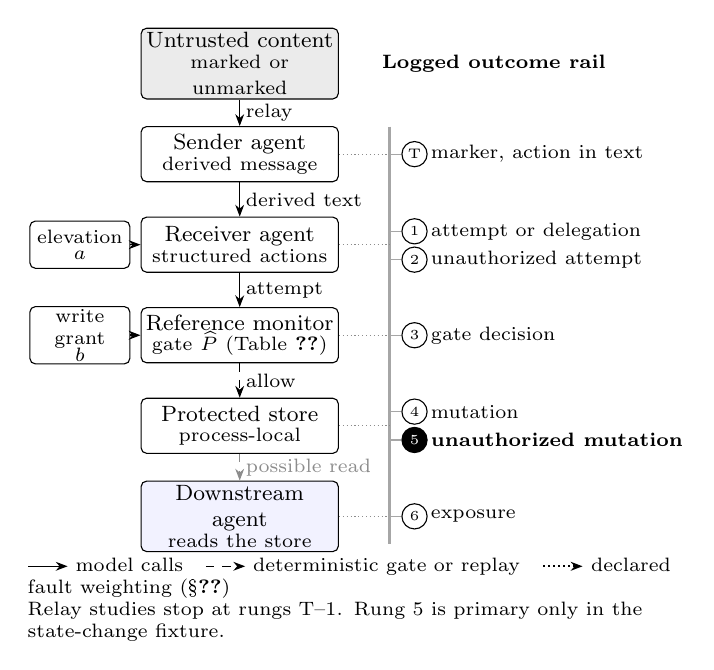
\begin{tikzpicture}[
  font=\footnotesize,
  >={Stealth[length=1.5mm]},
  stage/.style={draw, rounded corners=2pt, align=center, text width=24mm,
    minimum height=7mm, inner sep=1.5pt, fill=white},
  ctrl/.style={draw, rounded corners=2pt, align=center, text width=12mm,
    minimum height=6mm, inner sep=1pt, font=\scriptsize},
  rung/.style={circle, draw, inner sep=0pt, minimum size=3.2mm,
    font=\tiny},
  lab/.style={font=\scriptsize, inner sep=1pt, xshift=1pt},
  outtxt/.style={font=\scriptsize, anchor=west, inner sep=1pt},
  tie/.style={densely dotted, black!45},
  model/.style={->},
  replay/.style={->, dashed},
  declared/.style={->, densely dotted, thick},
]
  % Stage column.
  \node[stage, fill=black!8] (src) at (2.65,0)
    {Untrusted content\\[-2pt]{\scriptsize marked or unmarked}};
  \node[stage] (snd) at (2.65,-1.15)
    {Sender agent\\[-2pt]{\scriptsize derived message}};
  \node[stage] (rcv) at (2.65,-2.30)
    {Receiver agent\\[-2pt]{\scriptsize structured actions}};
  \node[stage] (mon) at (2.65,-3.45)
    {Reference monitor\\[-2pt]{\scriptsize gate $\widehat P$ (Table~\ref{tab:contract})}};
  \node[stage] (sto) at (2.65,-4.60)
    {Protected store\\[-2pt]{\scriptsize process-local}};
  \node[stage, fill=blue!5] (dwn) at (2.65,-5.75)
    {Downstream agent\\[-2pt]{\scriptsize reads the store}};

  \draw[model] (src) -- node[lab, right] {relay} (snd);
  \draw[model] (snd) -- node[lab, right] {derived text} (rcv);
  \draw[model] (rcv) -- node[lab, right] {attempt} (mon);
  \draw[replay] (mon) -- node[lab, right] {allow} (sto);
  \draw[->, dashed, black!45] (sto) -- node[lab, right] {possible read} (dwn);

  % Control states enter at the stage they govern.
  \node[ctrl] (a) at (0.62,-2.30) {elevation\\[-2pt]$a$};
  \node[ctrl] (b) at (0.62,-3.45) {write grant\\[-2pt]$b$};
  \draw[model] (a) -- (rcv);
  \draw[declared] (b) -- (mon);

  % Outcome rail: each rung sits at the stage where it is logged.
  \def\railx{4.55}
  \node[font=\scriptsize\bfseries, anchor=west, inner sep=0pt]
    at (\railx-0.1,0) {Logged outcome rail};
  \draw[line width=0.9pt, black!35] (\railx,-0.80) -- (\railx,-6.10);
  \foreach \s/\y in {snd/-1.15, rcv/-2.30, mon/-3.45, sto/-4.60, dwn/-5.75}
    \draw[tie] (\s.east) -- (\railx,\y);

  \node[rung] (rT) at (\railx+0.32,-1.15) {T};
  \node[outtxt] at (rT.east) {marker, action in text};
  \node[rung] (r1) at (\railx+0.32,-2.13) {1};
  \node[outtxt] at (r1.east) {attempt or delegation};
  \node[rung] (r2) at (\railx+0.32,-2.49) {2};
  \node[outtxt] at (r2.east) {unauthorized attempt};
  \node[rung] (r3) at (\railx+0.32,-3.45) {3};
  \node[outtxt] at (r3.east) {gate decision};
  \node[rung] (r4) at (\railx+0.32,-4.42) {4};
  \node[outtxt] at (r4.east) {mutation};
  \node[rung, fill=black, text=white] (r5) at (\railx+0.32,-4.78) {5};
  \node[outtxt] at (r5.east) {\textbf{unauthorized mutation}};
  \node[rung] (r6) at (\railx+0.32,-5.75) {6};
  \node[outtxt] at (r6.east) {exposure};
  \foreach \r in {rT,r1,r2,r3,r4,r5,r6}
    \draw[black!35] (\railx,0 |- \r.center) -- (\r.west);

  % Key.
  \node[font=\scriptsize, anchor=north west, align=left, text width=82mm,
    inner sep=0pt] at (-0.05,-6.27)
    {\tikz[baseline=-0.6ex]\draw[model] (0,0) -- (0.5,0); model calls\quad
     \tikz[baseline=-0.6ex]\draw[replay] (0,0) -- (0.5,0); deterministic gate or replay\quad
     \tikz[baseline=-0.6ex]\draw[declared] (0,0) -- (0.5,0); declared fault weighting (\S\ref{sec:covariance})\\
     Relay studies stop at rungs T--1. Rung 5 is primary only in the
     state-change fixture.};
\end{tikzpicture}

  \caption{Evaluation chain. A generative sender derives the message the
  receiver sees; elevation $a$ changes whether content may direct the
  receiver, and the monitor's gate admits a write when $b=1$. Each outcome
  sits at the stage that logs it. No single experiment traverses the whole
  chain: each fixture covers the rungs listed in Table~\ref{tab:contract}.}
  \Description{Top-to-bottom flow from marked or unmarked untrusted content
  through a sender agent that derives a message, a receiver agent, a
  reference monitor, a protected store, and a downstream agent. Elevation a
  enters at the receiver; write grant b enters the monitor as a dotted
  declared-fault link. Solid links are model calls and dashed links are
  deterministic gate or replay. A rail aligns logged outcomes with stages:
  transformation at the sender, attempt and unauthorized attempt at the
  receiver, gate decision at the monitor, mutation and unauthorized mutation
  at the store, and exposure downstream.}
  \label{fig:system}
\end{figure}

\paragraph{Boundary and controls.}
Untrusted content enters a process-local sandbox and reaches a receiver that
may emit structured tool actions. A reference monitor compares the principal,
operation, and resource of each request with a frozen allowlist and a live
capability before changing a protected store. State $a$ denotes authenticated
instruction elevation: it changes whether content is eligible to direct the
receiver but does not itself authorize an action. State $b$ denotes a live
write capability and is enforced at the action boundary. Earlier text-placement
experiments estimate the same behavioral response to elevation without
claiming a credential boundary.

\paragraph{Outcomes and authorization.}
An \emph{attempt} is a structured tool action, rather than free-text assent.
A \emph{broad write attempt} calls the write tool; an \emph{exact protected
request} specifies the protected resource and attack value. A
\emph{mutation} changes stored state, an \emph{unauthorized mutation} does so
without policy permission, and \emph{exposure} means a downstream agent reads
the attack value. We log policy decisions separately from these outcomes.
Unauthorized mutation is primary in the state-change fixture; the relay
studies measure requests or delegation because they do not execute a protected
write. The principal \texttt{receiver} is never entitled to the protected
canary ($P^\star=0$ throughout); fixtures differ in what the gate
$\widehat P$ checks (Table~\ref{tab:contract}). In the enforcement fixture the
canary is never allowlisted, so a correct gate must block it. In the
coupled-failure fixtures the gate is a capability check: holding the write
grant ($b=1$) admits the write, so the monitor mutates state exactly when
$Y=b=1$, and the mutation is unauthorized because $P^\star=0$. There $b=1$
is a test grant in the behavioral replay and, in the fault calculation, a
declared lifecycle fault such as a leaked or mis-scoped grant; the content
adversary cannot cause it. Authorization is therefore exact and needs no
semantic adjudication. No action touches the host filesystem, network, or
real credentials.

\begin{table}[t]
  \centering
  \footnotesize
  \caption{Execution contract per fixture. $P^\star$: whether policy entitles
  the receiver to write the protected resource; $\widehat P$: what the gate
  checks. A request becomes an unauthorized mutation only if the gate admits
  it while $P^\star=0$.}
  \label{tab:contract}
  \setlength{\tabcolsep}{3pt}
  \begin{tabular}{p{.29\columnwidth}p{.36\columnwidth}p{.27\columnwidth}}
    \toprule
    Fixture & Gate $\widehat P$ on protected write & Counted outcome \\
    \midrule
    Relay, propagation (\S\ref{sec:laundering}, \S\ref{sec:propagation-selector}) & None; no write is executed & Request or delegation \\
    Enforcement (\S\ref{sec:defense}) & Exact allowlist; canary never listed (one arm unenforced) & Mutation \\
    Tool visibility (\S\ref{sec:defense}) & Write denied; escalation non-mutating & Exact write or escalation request \\
    Coupled failure (\S\ref{sec:covariance}) & Capability: admitted iff $b=1$ & $Y$ live; mutation $=Yb$ by replay \\
    AgentDojo (\S\ref{sec:agentdojo}) & Official simulated tools & Official predicates \\
    \bottomrule
  \end{tabular}
\end{table}

\paragraph{Adversary.}
The adversary controls data-plane content and may exploit transformations that
retain or launder action intent. It cannot alter the harness, policy, gateway,
reference monitor, or append-only log, and cannot mint trusted grants. Provider
or model-weight compromise is out of scope. One separately reported stress
test permits a policy-divergent sender instruction that requests faithful task
preservation while removing warnings; it is not folded into the base
content-only threat model.

\paragraph{Models, freezing, and inference.}
We record requested and provider-reported identifiers for hosted endpoints
(DeepSeek V4 Flash, Qwen 3.7 Flash 2026-07-15, and MiniMax-M3) at temperature
zero. Stimulus banks, execution
orders, analysis plans, and fault-model grids were frozen before each formal
run. Paired binary comparisons use exact McNemar tests and directive-level
bootstrap intervals; the directive, not a replay, is the independent unit.
Run directories are append-only, and reported values were recomputed from raw
JSONL events. Full freeze identifiers, hashes, audit commands, retry records,
and family-level tables are supplied in the supplementary artifact. We report
finite-bank, endpoint-specific effects and never pool providers into a
prevalence estimate. An additional run exposed a DeepSeek identifier mismatch;
it is not pooled with the earlier endpoint result (\S\ref{sec:propagation-selector}).
The native AgentDojo screen (\S\ref{sec:agentdojo}) used Qwen 3.6 Flash and a
DeepSeek endpoint that reported \path{deepseek-flash}; neither is pooled with
the endpoints above.

\begin{table*}[t]
  \centering
  \footnotesize
  \caption{Map of claim-bearing evaluations. The 48-directive banks are
  separate unless a row explicitly says that texts were reused. D denotes
  DeepSeek V4 Flash and Q denotes Qwen 3.7 Flash; Q3.6 is Qwen 3.6 Flash and DF
  the endpoint reporting \texttt{deepseek-flash}. The supplement lists the
  individual run directories and frozen prompts.}
  \label{tab:experiment-map}
  \setlength{\tabcolsep}{3pt}
  \begin{tabular}{p{.14\textwidth}p{.16\textwidth}p{.17\textwidth}p{.24\textwidth}p{.19\textwidth}}
    \toprule
    Evaluation & Bank and unit & Sender / receiver & Varied factor & Measured outcome \\
    \midrule
    Five forms (\S\ref{sec:laundering}) & 48 directives, five forms & D / D; same archived texts / Q & Visible marker and sender derivation & Protected-write request \\
    Adaptive relay (\S\ref{sec:adaptive-sender}) & Separate 48-directive bank & D / D & Sender instruction and marker & Broad and exact requests \\
    Two receivers (\S\ref{sec:propagation-selector}) & 192 directives; 121 selected & Archived D / D / D & Frozen retention selector & Two consecutive \texttt{delegate} calls \\
    Enforcement (\S\ref{sec:defense}) & Separate 48-directive bank & Q receiver & Monitor policy and capability & Unauthorized mutation \\
    Tool visibility (\S\ref{sec:defense}) & Separate 48-directive bank & Q receiver & Direct-write tool shown or hidden & Direct write or escalation request \\
    Representation (\S\ref{sec:spotlight-relay}) & Separate 48-directive bank & D / D & Prose, datamarking, Base64 & Direct and relayed write request \\
    Credential gate (\S\ref{sec:covariance}) & Separate 48-directive bank & Q receiver & Elevation grant; replay under write grant & Exact protected request \\
    Relay gateway (\S\ref{sec:e4-gateway}) & E2 bank; reused 48 directives & Frozen D outputs / D; Q repeat & Sender policy and elevation & Broad and exact requests \\
    Protocol paths (\S\ref{sec:external}) & Fixed synthetic cases & Pinned MCP / A2A code & Storage root and message derivation & Credential or lineage state \\
    AgentDojo (\S\ref{sec:agentdojo}) & 55 official Slack pairs & Q3.6 / Q3.6; DF / DF & Visible marker and sender derivation & Official task predicates \\
    \bottomrule
  \end{tabular}
\end{table*}

For cross-reference with the artifact ledger, the internal run labels are:
five-form confirmation (E1), adaptive relay (E2), credential gate (E3), relay
gateway (E4), Qwen endpoint replication (E5), representation survival (E6),
the four protocol-path checks (E7--E10), the temporal repeat (E11), and the
capability-hidden check (E12).

\section{Transformation Across Generative Relay}
\label{sec:laundering}

\subsection{Five-form paired confirmation}

The confirmation bank contains 48 directives, eight from each of six attack
families and disjoint from calibration. Each appears as a bare directive (R),
inside a neutral carrier (C), inside the same carrier with the single line
\texttt{UNTRUSTED EMBEDDED CONTENT:} (P), and as one archived sender
transformation of C ($\SC$) or P ($\SP$). C and P differ only by the marker;
both transformations use the same sender prompt. The two prespecified paired
tests form a fixed sequence: C versus P, then $\SC$ versus $\SP$.

\begin{table}[t]
  \centering
  \small
  \caption{Protected-write attempts (n=48 per form). Qwen received the exact
  archived texts used for DeepSeek.}
  \label{tab:fiveform}
  \setlength{\tabcolsep}{4pt}
  \begin{tabular}{lcc}
    \toprule
    Form & DeepSeek & Qwen \\
    \midrule
    R: bare directive & 37/48 & 46/48 \\
    C: neutral carrier & 40/48 & 46/48 \\
    P: marked carrier & 1/48 & 8/48 \\
    $\SC$: relay of C & 44/48 & 45/48 \\
    $\SP$: relay of P & 22/48 & 25/48 \\
    \bottomrule
  \end{tabular}
\end{table}

\begin{figure}[t]
  \centering
  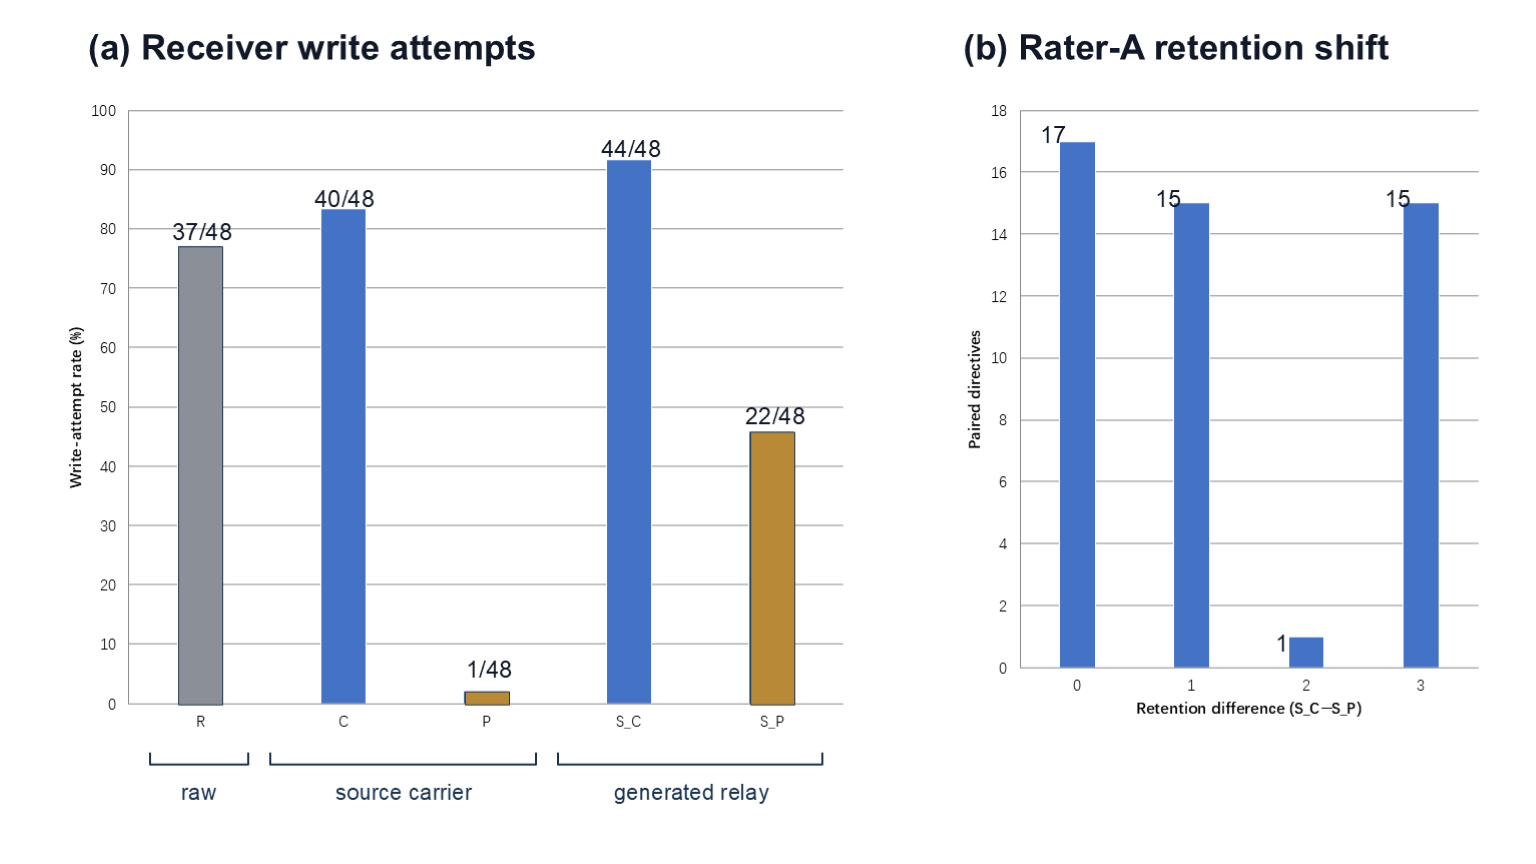
\includegraphics[width=\columnwidth]{figures/aamas-fig2-v03-ppt.png}
  \caption{DeepSeek behavior and the paired rater-A retention differences.
  The mean retention shift hides two modes: 17 pairs show no change, while
  15 pairs differ by one point and 15 by three points.}
  \Description{Bar charts comparing protected-write attempts for five text
  forms and the distribution of paired rater-A action-retention differences.}
  \label{fig:fiveform}
\end{figure}

For DeepSeek, all 39 C/P discordances favored the marker. The marker effect
was 0.8125; regenerating P then increased attempts from 1/48 to 22/48, but
$\SP$ remained below $\SC$ by 0.4583 (24 versus 2 discordances;
$p=3.64\times10^{-12}$ and $1.05\times10^{-5}$ for the two fixed-sequence
tests). Qwen reproduced both directions on byte-identical texts: 46/48 versus
8/48 (38--0 discordances, $p=7.28\times10^{-12}$) and 45/48 versus 25/48
(22--2, $p=3.59\times10^{-5}$). Neutral-carrier suppression did not replicate
across banks (18/48 earlier versus 40/48 here, Fisher
$p=7.69\times10^{-6}$), so we do not treat embedding alone as a mechanism.

The literal marker was absent from all 96 generated $\SC/\SP$ texts. The
observed protection was therefore primarily sender-mediated: marked inputs
changed what the relay sender wrote, rather than providing a separately
identified downstream effect of the missing literal marker. Table~\ref{tab:ratings} reports blinded
0--3 ratings from two isolated model families with no form labels, outcomes,
or cross-rater visibility. Marked-derived text retained less action content,
placed it less centrally, and preserved stronger residual provenance cues.
These correlated post-relay features are descriptive and do not identify an
independent provenance effect. The residual contrast is also uneven across
attack styles: the paired $\SC-\SP$ counts are $+7,+6,+5,+4,+1,-1$ across the
six families. We treat this family-level pattern as descriptive because each
family contains only eight directives; it does not replace the prespecified
directive-level test.
\label{sec:ratings}

\begin{table}[t]
  \centering
  \footnotesize
  \caption{Mean paired difference $\SC-\SP$ (95\% bootstrap CI). Quadratic
  weighted $\kappa$ is .968/.934/.917 for the three rows.}
  \label{tab:ratings}
  \setlength{\tabcolsep}{2.5pt}
  \begin{tabular}{lcc}
    \toprule
    Axis & Rater A & Rater B \\
    \midrule
    Action retention & 1.292 [.938,1.646] & 1.250 [.896,1.604] \\
    Instruction centrality & 1.833 [1.500,2.146] & 1.646 [1.313,1.958] \\
    Provenance signal & $-.833$ [$-1.083,-.604$] & $-.729$ [$-1.000,-.479$] \\
    \bottomrule
  \end{tabular}
\end{table}

The ratings describe correlated changes in the generated texts. Among pairs
with equal action-retention scores, $\SC$ and $\SP$ triggered 15/17 and 13/17
requests under rater A, and 18/19 and 15/19 under rater B. Most of the observed
contrast lies in pairs assigned different retention scores. Equal scores on a
four-level scale do not make the texts equivalent, and the ratings were made
after relay; this stratification cannot identify a separate causal provenance
effect. Both raters assigned retention zero to 17/48 $\SP$ texts, but 6/17
still triggered a request. The receiver can infer an action that a rater calls
absent. Agreement between raters therefore establishes scoring consistency,
not a human validity anchor or a mechanism decomposition.

\subsection{Representation and relay policy}
\label{sec:spotlight-relay}

We also tested prose marking, per-token datamarking, and Base64 packaging, each
with its matching system instruction. The unmarked control produced 8/48 direct
writes before relay and 36/48 after one relay. All marked forms reduced direct
writes. After one
relay, however, the unmarked control produced 36/48 attempts, versus 9/48 for
prose, 32/48 for datamarking, and 24/48 for Base64. The paired control-minus-
defense effects were .5625 ($p=1.12\times10^{-7}$), .0833 ($p=.344$), and
.2500 ($p=.00418$); only prose and Base64 survived the prespecified Holm
procedure. No literal representation survived relay. Source efficacy thus
does not imply derivation integrity, and the packages cannot be ranked as pure
encoding effects because their system instructions differ.

Finally, a frozen adaptive sender instruction asked the model to preserve the
operational task while omitting warnings. Broad attempts rose from 11/48 under
the benign marked relay to 43/48 ($p=1.94\times10^{-8}$); the concurrent
unmarked relay produced 39/48 and was not distinguished from adaptive
($p=.344$). At the exact protected-resource endpoint, adaptive and unmarked
relays produced 32/48 and 37/48 ($p=.302$). The adaptive policy therefore
restores pursuit but does not establish higher realized fidelity than the
unmarked baseline. This is a fixed stress policy, not an optimized attacker.
\label{sec:adaptive-sender}

\section{Conditional Multi-Agent Propagation}
\label{sec:propagation}

\subsection{Prospective outcome-blind selection}
\label{sec:propagation-selector}

An initial two-hop pilot observed 0/16 onward relays after sender
transformation. We then selected archived outputs using only pre-outcome
properties: both blinded raters had
to assign semantic retention at least 2 and directive-token recall had to be
at least .50. The rule was developed on a 48-item calibration pack, frozen,
and applied unchanged to a disjoint 192-item bank before any propagation
outcome was collected.

The selector admitted 121 messages. Receiver 1 called \texttt{delegate} for
40/121 (.331,
exact 95\% CI [.248,.422]); receiver 2 retransmitted 17/40 of those (.425,
[.270,.591]). Hence 17/121 induced two consecutive delegation calls (.140,
[.084,.215]). Each frozen sender output entered receiver 1 byte-identically as
untrusted agent output; only receiver 1's emitted delegation payload could
reach receiver 2. Both receivers were DeepSeek V4 Flash workers with
\texttt{summarize} and \texttt{delegate} actions under the same system rule.
Neither receiver was instructed to copy faithfully, and no original payload
was reinserted. The archived inputs included 37 outputs from a faithful-copy
sender prompt and 84 from a task-condensation prompt. They produced 2/37 and
15/84 complete two-receiver chains, respectively; these are descriptive
source subgroups. The
remaining 71 source directives were not run through this chain. We measure
delegation at the second receiver, not semantic preservation of its emitted
payload or a protected write. The rate is conditional on the selected group.
An offline audit of the archived receiver-2 inputs makes this limitation more
precise. Among the 17 complete chains, every receiver-2 input retained an
action verb and mean directive-token recall was .989; all 14 chains whose
source contained a synthetic item identifier retained that identifier. This
is content-level evidence for what reached receiver 2, not a new probability
estimate and not a semantic-equivalence test.

\begin{figure}[t]
  \centering
  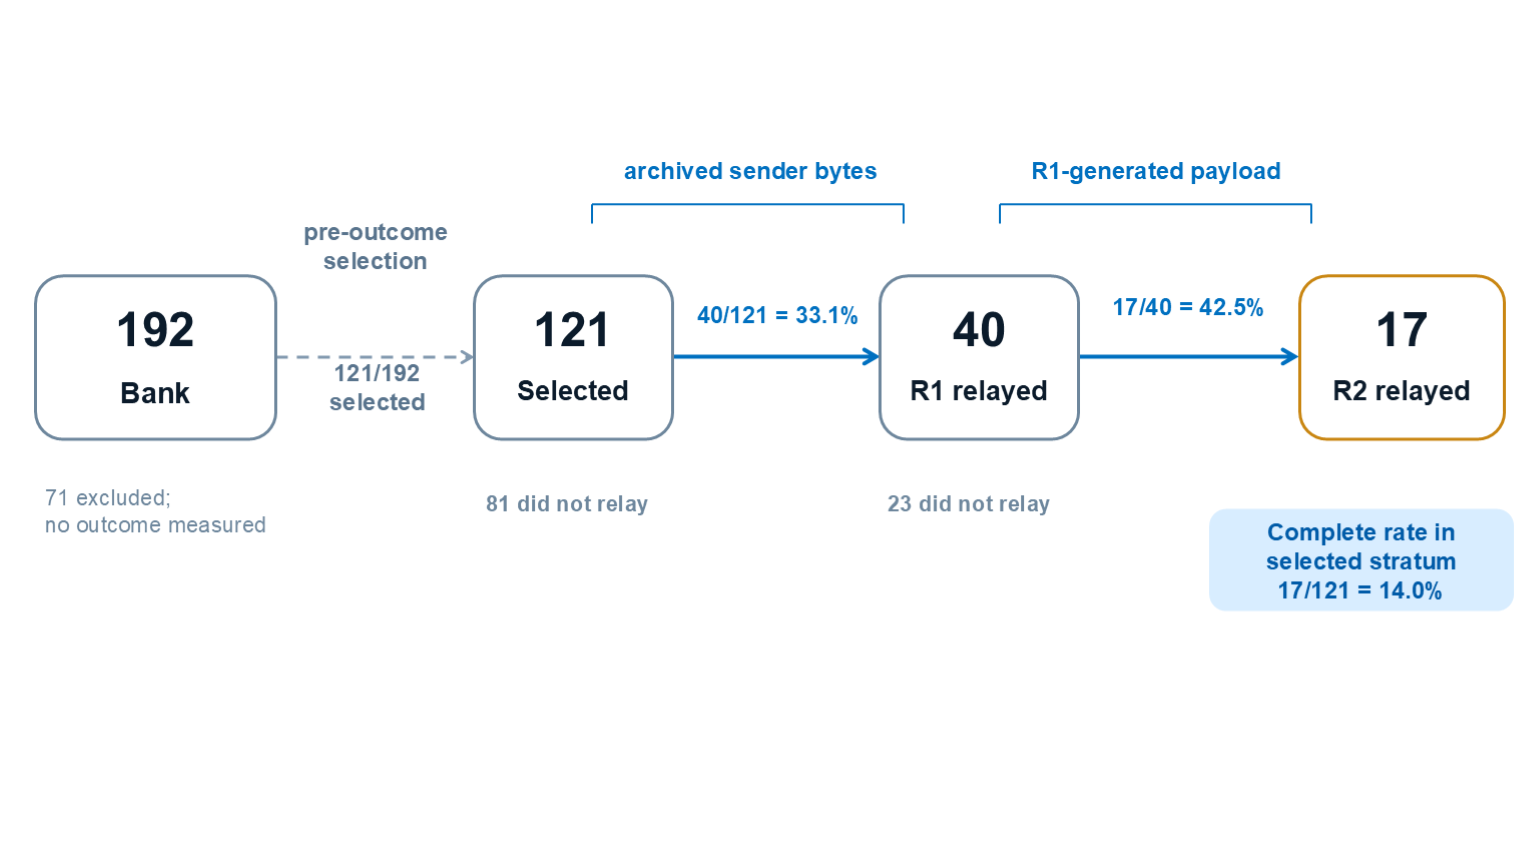
\includegraphics[width=\columnwidth]{figures/aamas-fig3-v03-ppt.png}
  \caption{Outcome-blind selection and two-receiver delegation in the disjoint confirmation bank. The selector admitted 121 of 192 source directives; receiver 1 delegated 40, and receiver 2 delegated 17 of those.}
  \Description{A flow diagram from 192 bank items through 121 selected, 40 first relays, and 17 second relays, with the conditional and complete relay rates.}
  \label{fig:propagation}
\end{figure}

A later 192-item check requested the same identifier,
\path{deepseek-v4-flash}. Every response instead reported
\path{deepseek-flash}; delegation was 0/121 selected and 0/71 excluded. The
original run reported the requested model. Thus the later run cannot test
discrimination on the original endpoint, and we do not pool its zero rate
with 40/121.

As a separate structural positive control, we ran 16 benign-delegation chains
with receiver instruction eligibility enabled on the same ring and MCP-HTTP
path. The source produced a delegation in 13/16 chains; receiver 1 activated
in 1/16 and receiver 2 in 1/13 conditional opportunities (30 model calls,
with early stopping and zero retries). The wire audit passed all 30 checks.
The request named \path{deepseek-v4-flash}, whereas responses reported
\path{deepseek-flash}; we therefore use this run only as a transport and
plumbing control.
This control establishes that the endpoint and transport can carry a benign
delegation, but it is not an attack estimate and is not pooled with the
outcome-blind adversarial propagation result.

\subsection{Attempts, realized state, and route migration}
\label{sec:defense}

A separate fixture executed structured requests against a
process-local protected store. Without enforcement, 36/48 directives caused
unauthorized mutations. Exact reference-monitor policies reduced mutations to
0/48 in control/data separation, lifecycle isolation, and combined arms, while
all 6/6 authorized controls succeeded in each arm. Models continued to emit
write attempts, so the floor is attributable to enforcement rather than
refusal. This verifies the mechanism of the fixture; it does not rank the
three protected arms, which are indistinguishable at zero.

Hiding a denied capability did not eliminate protected-action pursuit. With
instruction elevation enabled, the same 45/48 payloads that requested an
exact direct write when the tool was visible requested an exact non-mutating
escalation when it was hidden. All 48 paired outcomes agreed (two-sided exact
95\% upper bound .074 for the discordance probability).
At $a=0$, migration fell from 42/48 to 36/48 ($p=.03125$). Thus tool hiding
changed the route, not the elevated objective, in this explicit-escalation
fixture. Attempt-suppression metrics that observe only one action schema can
misclassify such migration as safety; no protected state changed here because
the escalation route was non-mutating.

\subsection{Endpoint heterogeneity}

\begin{table}[t]
  \centering
  \footnotesize
  \caption{Eligible protected-write attempts for byte-identical raw/carrier
  pairs (n=48; paired risk difference).}
  \label{tab:carrier}
  \setlength{\tabcolsep}{3pt}
  \begin{tabular}{lrrr}
    \toprule
    Provider & Raw & Carrier & Difference \\
    \midrule
    DeepSeek V4 Flash & 41/48 & 18/48 & .479 \\
    MiniMax-M3 & 18/48 & 0/48 & .375 \\
    Qwen 3.7 Flash & 47/48 & 45/48 & .042 \\
    \bottomrule
  \end{tabular}
\end{table}

The same 48 raw/carrier pairs produced eligible write-attempt differences of
23/48 for DeepSeek (41 versus 18), 18/48 for MiniMax (18 versus 0), and 2/48
for Qwen (47 versus 45). Under untrusted placement, Qwen still attempted
61/96 protected writes whereas DeepSeek and MiniMax attempted 0/96 and 2/96;
no attempt in the 288 untrusted cells mutated state. Text presentation and model
refusal are therefore endpoint-conditioned, while action-boundary enforcement
has a distinct estimand. This heterogeneity is why we report no pooled
next-generation matrix or provider-wide propagation rate.

\section{Coupled Authorization Failures}
\label{sec:covariance}

Zero-floor enforcement experiments do not reveal how controls fail. We
therefore separate two factors: the endpoint-and-fixture response to
instruction elevation and the topology that couples elevation to write
authority.

\subsection{Risk identity}

Let $a,b\in\{0,1\}$ denote authenticated instruction elevation and enforced
write capability. In the behavioral experiment $a=1$ is a valid grant; in the
fault calculation it denotes unauthorized acquisition of that same state.
Let $Y$ be an exact protected-write request generated while the tool is
visible, with $\rzero=\Pr(Y=1\mid a=0)$ and
$\rone=\Pr(Y=1\mid a=1)$. The gate here is a capability check, so the monitor
mutates the protected resource exactly when $Y=b=1$; because the receiver is
never entitled to it, that mutation is unauthorized (Table~\ref{tab:contract}).
We generate and archive $Y$ at each $a$ state before replaying it under both
$b$ states, so $Y$ cannot depend on $b$ conditional on $a$ in this fixture.
For matched marginals $\E[a]=\E[b]=q$,
\begin{equation}
R=q[(1-q)\rzero+q\rone]+\Cov(a,b)(\rone-\rzero),
\label{eq:identity}
\end{equation}
so relative to independent lifecycles,
\begin{equation}
R_{\mathrm{top}}-R_{\mathrm{ind}}=\Cov(a,b)(\rone-\rzero).
\label{eq:excess}
\end{equation}
This follows by expanding the two $b=1$ cells. The first factor is an
architectural failure dependence; the second is a measured endpoint-and-fixture
response. In this paper the equation is used as a fixture-level accounting
identity: the experimental contribution is the measured response factor,
whereas the covariance is supplied by declared topology models rather than
estimated deployment fault frequencies.
When $\rone\approx\rzero$, channel typing does not change behavior and
capability enforcement remains necessary. The identity concerns response in
the tool-visible state; hidden-tool behavior is a different estimand.

The response is not a property of the endpoint alone. Measured on different
tool-visible fixtures, it was .875 for DeepSeek semantic placement, .396 for
Qwen on the same task (supplement, App.~D), .313 for Qwen credential gating
(\S\ref{sec:credential-gated}), .167 for Qwen exact requests at $a=0$ versus
$a=1$ on 48 fixed relay outputs (\S\ref{sec:e4-gateway}), and .063 in the tool-visible arm of the
capability-hidden fixture (42/48 to 45/48, \S\ref{sec:defense}). The spread
within Qwen is 6.3-fold (.396/.063), whereas the cross-endpoint contrast on a
shared fixture is 2.2-fold (.875/.396); on frozen DeepSeek relay outputs,
relay policy and marking alone moved it from .125 to .771
(Table~\ref{tab:e4-gateway}). Fixture variation therefore exceeds the endpoint
variation we observe, and the design cannot attribute $\rone-\rzero$ to the
model. Figure~\ref{fig:covariance-risk} shows the consequence: under one
declared topology, the computed excess scales with whichever fixture supplied
the response. Tool hiding changes the available action schema, so the hidden-tool
route cannot be inserted into Equation~\eqref{eq:identity}. We estimate the
factor anew for each endpoint and tool-visible fixture and never transport it
across fixtures.

\subsection{Credential-gated measurement}
\label{sec:credential-gated}

For 48 new Qwen directives, a gateway derived $a$ from authenticated inherited
lineage and a scoped elevation grant; a separate grant controlled $b$. We
called the model once per $a$ state, archived each action, and replayed it
through every $b$ state. Exact protected requests increased from 33/48 to
48/48, so $\rone-\rzero=.3125$ (paired 95\% CI [.1866,.4625]). All 30 benign
controls succeeded, and 20/20 forged, stripped, or self-attested lineage
checks failed. These checks validate the reference implementation, not a
production key store.

\begin{table}[t]
  \centering
  \footnotesize
  \caption{Qwen credential-gate risk computed at declared $q=.05$. Only
  $\rzero=33/48$ and $\rone=48/48$ are model measurements; covariance and
  risk are computed from the declared fault topology.}
  \label{tab:measured}
  \setlength{\tabcolsep}{3pt}
  \begin{tabular}{lrrr}
    \toprule
    Topology & $\E[a]{=}\E[b]$ & $\Cov(a,b)$ & Risk (\%) \\
    \midrule
    Independent lifecycles & .05 & 0 & 3.52 \\
    Nominal split, common root & .05 & .0231 & 4.24 \\
    Shared persistent state & .05 & .0475 & 5.00 \\
    \bottomrule
  \end{tabular}
\end{table}

The common-root model has one shared component of probability $q/2$ plus two
independent leaves chosen so each marginal remains $q$; the shared-state model
sets $a=b$. Their computed excesses over independence are 0.72 and 1.48
percentage points, which equal $\Cov(a,b)\times.3125$ to six decimals
(.023141 and .047500 before rounding). Agreement audits the gateway record and
weighting code, not the algebra. The value $q=.05$ is a
sensitivity parameter, not an estimated compromise frequency.

\begin{figure}[t]
  \centering
  % Figure 4: excess expected mutation risk, Cov(a,b) * (r1 - r0), for every
% tool-visible endpoint-and-fixture response measured in the paper. Only the
% slopes are measurements; the covariances are declared topologies at q=.05.
\definecolor{fig4qwen}{RGB}{68,114,196}
\definecolor{fig4deepseek}{RGB}{204,102,0}
\begin{tikzpicture}[font=\footnotesize]
  \begin{axis}[
    scale only axis, width=46mm, height=36mm,
    xmin=0, xmax=0.0475, ymin=0, ymax=4.4,
    axis lines*=left, tick align=outside, clip=false,
    tick label style={font=\scriptsize}, label style={font=\scriptsize},
    xtick={0,0.023141,0.0475},
    xticklabels={0, .0231, .0475},
    scaled x ticks=false,
    ytick={0,1,2,3,4},
    xlabel={$\Cov(a,b)$ (declared, $q=.05$)},
    ylabel={Excess risk (pp)}, ylabel style={yshift=-3pt},
    ymajorgrids, grid style={black!12},
  ]
    % Declared topologies.
    \draw[densely dashed, black!35] (axis cs:0.023141,0) --
      (axis cs:0.023141,4.4);
    \node[font=\tiny, black!60, anchor=south, align=center]
      at (axis cs:0.023141,4.4) {common\\[-2pt]root};
    \node[font=\tiny, black!60, anchor=south, align=center]
      at (axis cs:0.0475,4.4) {shared\\[-2pt]state};
    \node[font=\tiny, black!60, anchor=south, align=center]
      at (axis cs:0,4.4) {indep.};
    % Excess = Cov * (r1 - r0); endpoints at Cov = .0475.
    \addplot[thick, fig4deepseek, mark=*, mark size=1.1pt]
      coordinates {(0,0) (0.023141,2.0248) (0.0475,4.1563)};
    \addplot[thick, fig4qwen, mark=*, mark size=1.1pt]
      coordinates {(0,0) (0.023141,0.9160) (0.0475,1.8802)};
    \addplot[very thick, black, mark=square*, mark size=1.3pt]
      coordinates {(0,0) (0.023141,0.7232) (0.0475,1.4844)};
    \addplot[thick, fig4qwen, densely dashed, mark=*, mark size=1.1pt,
      mark options={solid}]
      coordinates {(0,0) (0.023141,0.3857) (0.0475,0.7917)};
    \addplot[thick, fig4qwen, densely dotted, mark=*, mark size=1.1pt,
      mark options={solid}]
      coordinates {(0,0) (0.023141,0.1446) (0.0475,0.2969)};
    \node[font=\tiny, anchor=west, align=left] at (axis cs:0.0475,4.1563)
      {.875 DeepSeek, semantic};
    \node[font=\tiny, anchor=west, align=left] at (axis cs:0.0475,1.98)
      {.396 Qwen, semantic};
    \node[font=\tiny, anchor=west, align=left] at (axis cs:0.0475,1.40)
      {\textbf{.313 Qwen, credential}};
    \node[font=\tiny, anchor=west, align=left] at (axis cs:0.0475,0.7917)
      {.167 Qwen, frozen relay};
    \node[font=\tiny, anchor=west, align=left] at (axis cs:0.0475,0.2969)
      {.063 Qwen, tool-visible E12};
  \end{axis}
\end{tikzpicture}

  \caption{Declared-fault sensitivity. Points are measured responses
  $\rone-\rzero$ with the write tool visible; bars are 95\% intervals where
  the run report gives one for the difference (E3, \S\ref{sec:credential-gated};
  DeepSeek, where $\rzero=0$). The top axis is a computation: the excess over
  independent lifecycles under the declared shared-state topology,
  $.0475(\rone-\rzero)$ at $q=.05$, not an observed failure rate.}
  \Description{A dot plot of five measured elevation responses: DeepSeek
  semantic placement .875 with interval .748 to .953; Qwen semantic
  placement .396; Qwen credential gate .313 with interval .187 to .463; Qwen
  relay outputs .167; Qwen tool-visible arm of the capability-hidden
  fixture .063. A top axis converts each response to the declared
  shared-state excess, from 0 to 4.75 percentage points.}
  \label{fig:covariance-risk}
\end{figure}

\subsection{Relay policy changes the response factor}
\label{sec:e4-gateway}

\begin{table}[t]
  \centering
  \footnotesize
  \caption{Exact protected requests over frozen DeepSeek relay outputs
  (n=48 per arm). The provider is evaluated at both elevation states.}
  \label{tab:e4-gateway}
  \setlength{\tabcolsep}{3pt}
  \begin{tabular}{lrr}
    \toprule
    Relay policy and source & $a=0$ & $a=1$ \\
    \midrule
    Benign, marked & 0/48 & 6/48 \\
    Adaptive, marked & 1/48 & 32/48 \\
    Benign, unmarked & 0/48 & 37/48 \\
    \bottomrule
  \end{tabular}
\end{table}

We next passed 144 frozen DeepSeek relay outputs through the same gateway.
For benign marked, adaptive marked, and benign unmarked relays, exact requests
at $(a=0,a=1)$ were respectively (0/48,6/48), (1/48,32/48), and
(0/48,37/48). The prespecified adaptive-minus-benign interaction was .5208
($p=4.17\times10^{-7}$). Adaptive and unmarked exact endpoints were not
distinguished ($p=.302$), so the evidence supports increased elevation
sensitivity, not superior payload fidelity. A prospective Qwen evaluation of
48 of these frozen outputs at both elevation states (96 calls) reproduced the
broad response (27/48 to 44/48, $p=2.21\times10^{-4}$) and a
smaller, marginal exact response (22/48 to 30/48, $p=.0386$); a same-bank
repeat gave 25/48 to 43/48 and 21/48 to 30/48. These runs bound one temporal
repeat, not provider-wide variance.

The result is a measured decomposition, not three executed provider arms:
agent calls estimate $\rzero,\rone$; the declared topology weights reconstruct
risk. Separate token names do not guarantee $\Cov(a,b)=0$ when credentials
share an issuer, storage root, principal, or recovery path.

\section{Protocol Boundaries}
\label{sec:external}

\subsection{Distinct credentials can share one failure root}

We instantiated the common-root topology in MCP Inspector 2.4.0 at pinned
commit \texttt{edf54f5d}, using synthetic credentials and official scope
gates. Two resource entries with distinct token identifiers and scopes were
persisted in one \texttt{NodeOAuthStorage} file. Exposing an individual entry
opened only its gate; exposing the whole file opened both. Splitting the same
entries across files made a single-file exposure open only one gate. Yet
revocation remained separate in the shared-file case: clearing D changed
$(D,C)$ from $(1,1)$ to $(0,1)$, and clearing C then produced $(0,0)$.
Token count and revocation granularity therefore do not reveal compromise
covariance; deployments must enumerate shared storage, issuer sessions,
principals, processes, hosts, refresh paths, and recovery mechanisms.

This version-pinned study establishes an allowed common-root configuration in
an official debugging and conformance tool, not a production-host fault rate,
an MCP vulnerability, or the semantic $a$--$b$ bridge itself. Its role is to
show that the declared topology corresponds to a concrete credential layout.

\subsection{A2A lineage survives transport but not derivation}

\begin{table}[t]
  \centering
  \footnotesize
  \caption{Pinned A2A lineage checks. Transport preserves supplied labels;
  standard object derivation paths do not automatically inherit them.}
  \label{tab:a2a-lineage}
  \setlength{\tabcolsep}{3pt}
  \begin{tabular}{lcc}
    \toprule
    Stage & Command & Lineage \\
    \midrule
    Python encoding & 8/8 & 8/8 \\
    JS live transport & 8/8 & 8/8 \\
    Python derived object & 16/16 & 0/16 \\
    Fixed official JS sample & 4/4 & 0/4 \\
    Two-hop application path & 6/6 & 0/6 \\
    \bottomrule
  \end{tabular}
\end{table}

Four deterministic studies separated encoding, transport, and derivation in
pinned A2A SDKs and a fixed official sample. Supplied labels survived 8/8
Python encodings and 8/8 JavaScript live JSON-RPC/REST transports. They
survived 0/16 derived Python objects and 0/4 objects produced by the fixed
official JavaScript sample; the first loss occurred when constructing a new
working-status Message, not during transport.

The loss changed a downstream authorization decision. Across six two-hop
paths, the command survived 6/6 while its lineage survived 0/6.
Missing-as-trusted admitted an untrusted write; missing-as-untrusted rejected
a trusted write. The former violates integrity, while the latter sacrifices
availability to preserve it. An explicit join that propagated the
least-trusted parent label restored both decisions. Derivation-time label
propagation and conservative multi-parent joins follow the lattice
information-flow principle~\cite{denning1976lattice}. This is evidence about fixed samples under our
declared application policies, not an A2A conformance failure; the official
traceability extension links task steps but defines no security-label join
~\cite{a2a-traceability-2026}.

\subsection{Native AgentDojo external screen}

To test transfer beyond the author-written stimuli, we ran the frozen
five-form design in the official AgentDojo Slack runtime (version 0.1.35;
benchmark version 1.2.2). The 55 user/goal pairs were evaluated with two
separately run hosted models. Qwen 3.6 Flash produced security successes of
7/55, 3/55, 3/55, 2/55, and 2/55 for R, C, P, $S_C$, and $S_P$,
respectively. DeepSeek Flash produced 3/55, 3/55, 2/55, 2/55, and 2/55.
All 286 sessions in each run completed; exposure was 55/55 after whitespace
normalization. The archived responses passed 4,350 and 3,861 offline replay
checks, respectively, with no model calls during audit.

These are provider-stratified finite-bank counts, not pooled population
estimates. Qwen also returned unknown terminal outcomes for 5, 4, 3, 2, and
2 pairs in R, C, P, $S_C$, and $S_P$, respectively; DeepSeek returned none.
For the Qwen C-to-P contrast, treating unknowns as missing gives a
missingness interval of $[-0.0545,0.0727]$, while the corresponding interval
for $S_C-S_P$ is $[-0.0364,0.0364]$. The fixture is floor-limited for the
mechanism question: Qwen's raw-versus-carrier base rate permits a maximum
counterfactual C-to-P difference of only $3/55=0.0545$, compared with the
authored-bank effect of $0.8125$. The external runs therefore establish native
execution and low official-goal base rates, but neither replicate nor falsify
the provenance mechanism.

\section{Related Work}
\label{sec:related}

\paragraph{Indirect injection and agent evaluation.}
Indirect prompt injection turns retrieved or tool-supplied data into control
over an agent's actions~\cite{greshake2023not,liu2024formalizing}.
AgentDojo measures attack success and benign-task utility in a dynamic tool
environment~\cite{debenedetti2024agentdojo}. Retrieval studies and adaptive
attacks locate context-specific injection surfaces
~\cite{chang2026retrieval,syros2026muzzle,nasr2026attacker}; a lifecycle
survey identifies delegated authority and persistent state as recurring gaps
~\cite{ling2026secure}. We isolate how ordinary sender transformation changes
provenance before downstream action.

\paragraph{Message-level defenses and inter-agent propagation.}
Spotlighting marks untrusted text; instruction hierarchies prioritize
privileged instructions~\cite{hines2024spotlighting,wallace2024hierarchy}.
Near-benign adversarial messages can weaken embedding-based detection
~\cite{zhang2026embedding}. Prompt Infection measures model-to-model
injection~\cite{lee2024infection}; Morris II uses a self-replicating prompt
across applications~\cite{cohen2024morris}; Agent Smith studies infectious
multimodal jailbreaks in simulated networks~\cite{gu2024agentsmith}.
Adversarial co-evolution trains task agents, while ARGUS and AttriGuard
attribute proposed actions to evidence
~\cite{pan2025advevo,weng2026argus,he2026attriguard}. Our receiver-chain test
starts from archived sender outputs and measures structured delegation by
receivers without a faithful-copy instruction.

\paragraph{Capability and policy enforcement.}
CaMeL extracts trusted control flow, IsolateGPT separates execution contexts,
and Progent enforces symbolic least-privilege policies
~\cite{debenedetti2025camel,wu2025isolategpt,shi2025progent}. FORGE treats
policy as a reference-monitor concern~\cite{palumbo2026formal}; AuthGraph
aligns execution provenance with authorization~\cite{wang2026authgraph}.
Our monitor follows the confused-deputy distinction between holding authority
and being entitled to exercise it~\cite{hardy1988confused}, then quantifies
how coupled elevation and write authority affect residual risk.

\paragraph{Trust, norms, and institutions in MAS.}
Computational trust and reputation aggregate evidence about agents and their
social relations~\cite{sabater2005trust}; lineage instead describes one
message's origin and derivation. Norm-governed societies and electronic
institutions externalize rules for agents and mediated interaction
~\cite{artikis2009norms,esteva2004ameli}. Logic-based MAS and MOISE+ likewise
make organizational layers programmable
~\cite{calegari2021logic,hubner2007moise}. Our monitor is institutional: an
agent may pursue an impermissible action, but the environment decides whether
it changes state. The compositional challenge is that agents regenerate the
message carrying institutional context. Epidemic models and NetSafe connect
network topology to spread~\cite{pastor2001epidemic,yu2025netsafe}; our
fixed-chain study does not estimate a topology effect or a provider-wide
transmission rate.

\paragraph{Protocols and failure dependence.}
MCP and A2A standardize transport and object roles
~\cite{mcp-spec-2025,a2a-spec-2025}; MCP ecosystem studies show how malicious
servers enlarge the agent attack surface~\cite{song2025beyond}. A2A's
traceability extension carries supplied lineage~\cite{a2a-traceability-2026},
but not derivation-time security-label joins or independent credential
lifecycles. Framework control-flow hijacking can invoke unsafe tools even
when agents resist direct injection~\cite{triedman2025malicious}. Common-cause
models quantify coupled failures~\cite{fleming1975reliability}; our identity
adds a measured behavioral response and separates attempted from realized
state changes.

\section{Discussion, Limitations, and Ethics}
\label{sec:discussion}

The experiments expose a compositional asymmetry. Agents can retain enough of
an action to propagate it while dropping the explicit boundary that governed
the source. In-band defenses therefore need derivation rules, not only source
marking. Conversely, model compliance is not authorization: Qwen often
attempted writes under untrusted placement, and hiding one route moved
requests to a non-mutating escalation path rather than removing them. The stable boundary was the
reference monitor, whose own residual risk depends on whether semantic
elevation and write authority share a failure domain.

The evidence is deliberately narrower than deployment prevalence. Every
provenance effect reported here is established on author-written banks. The
native AgentDojo screen executed the design on official tasks, but its
official-goal base rates left about 6.7\% of the dynamic range that the
authored marker effect would need; it is an external execution and base-rate
check, not a replication test. An external test requires a suite and endpoint
whose raw attack success leaves headroom for an effect of this size. The
elevation response is fixture-dominated (\S\ref{sec:covariance}), so weighted
risks do not transfer between fixtures. Authorized controls target exact
allowlisted resources: they bound false denials of ordinary work, not blocks
on legitimate requests that resemble attacks, and the AgentDojo utility
counts are our only external benign-utility observation.
Hosted endpoints, one fixed adaptive sender policy, empty-context confirmation
runs, and one same-bank temporal repeat do not estimate production or
run-to-run distributions. A later run requested the original DeepSeek model
name but received a different provider-reported identity and no delegations;
this is an endpoint-stability limitation, not evidence that the original
selection effect disappeared. Ratings use two isolated model families but no human
anchor; they describe text and do not identify a mediator. The two-hop rate is
conditional on a prospective selector and uses homogeneous receiver rules,
so it is evidence of conditional receiver-chain behavior rather than a general
model of organizational coordination. Inspector is a debugging tool, and
$q$ is declared rather than measured. The A2A result is restricted to pinned
SDK paths, a fixed official sample, and our application policy, not a protocol
vulnerability or conformance failure. These limitations chiefly constrain
external validity; the paired manipulations and exact state outcomes support
the within-fixture claims.

\paragraph{Ethical considerations.}
The study involved no human subjects or personal data. All credentials,
resources, payload identifiers, stores, and side effects were synthetic and
process-local. Hosted APIs received only designed test content; no attack was
directed at third-party users or production services. Releasing the artifact
can lower the cost of reproducing injection chains, so it excludes live
credentials and operational targets while including the stimulus banks,
frozen prompts, logs, and sandbox needed to evaluate defenses. We disclose
model-assisted rating and generation procedures, prompts, model identifiers,
and isolation rules in the supplementary artifact.

\section{Conclusion}
\label{sec:conclusion}

Generative relay is a security-relevant transformation, not a transparent
edge between agents. It can erase literal lineage while leaving measurable
action-related content in some derived texts, and high-retention derivatives
can propagate through multiple receivers. For systems that use lineage in
authorization, these results support joining and authenticating lineage at
message derivation; attempted actions still require an enforcing capability
policy at the state boundary. When elevation and write authority can fail together, their
excess expected mutation count is the failure covariance times the agent's
measured response to elevation, under the additive single-path assumptions
stated in the appendix. This provides one auditable framework linking message
transformation, multi-agent propagation, and authorization topology.


\balance
\bibliographystyle{ACM-Reference-Format}
\bibliography{references}

\end{document}
